\documentclass[1p]{elsarticle_modified}
%\bibliographystyle{elsarticle-num}

%\usepackage[colorlinks]{hyperref}
%\usepackage{abbrmath_seonhwa} %\Abb, \Ascr, \Acal ,\Abf, \Afrak
\usepackage{amsfonts}
\usepackage{amssymb}
\usepackage{amsmath}
\usepackage{amsthm}
\usepackage{scalefnt}
\usepackage{amsbsy}
\usepackage{kotex}
\usepackage{caption}
\usepackage{subfig}
\usepackage{color}
\usepackage{graphicx}
\usepackage{xcolor} %% white, black, red, green, blue, cyan, magenta, yellow
\usepackage{float}
\usepackage{setspace}
\usepackage{hyperref}

\usepackage{tikz}
\usetikzlibrary{arrows}

\usepackage{multirow}
\usepackage{array} % fixed length table
\usepackage{hhline}

%%%%%%%%%%%%%%%%%%%%%
\makeatletter
\renewcommand*\env@matrix[1][\arraystretch]{%
	\edef\arraystretch{#1}%
	\hskip -\arraycolsep
	\let\@ifnextchar\new@ifnextchar
	\array{*\c@MaxMatrixCols c}}
\makeatother %https://tex.stackexchange.com/questions/14071/how-can-i-increase-the-line-spacing-in-a-matrix
%%%%%%%%%%%%%%%

\usepackage[normalem]{ulem}

\newcommand{\msout}[1]{\ifmmode\text{\sout{\ensuremath{#1}}}\else\sout{#1}\fi}
%SOURCE: \msout is \stkout macro in https://tex.stackexchange.com/questions/20609/strikeout-in-math-mode

\newcommand{\cancel}[1]{
	\ifmmode
	{\color{red}\msout{#1}}
	\else
	{\color{red}\sout{#1}}
	\fi
}

\newcommand{\add}[1]{
	{\color{blue}\uwave{#1}}
}

\newcommand{\replace}[2]{
	\ifmmode
	{\color{red}\msout{#1}}{\color{blue}\uwave{#2}}
	\else
	{\color{red}\sout{#1}}{\color{blue}\uwave{#2}}
	\fi
}

\newcommand{\Sol}{\mathcal{S}} %segment
\newcommand{\D}{D} %diagram
\newcommand{\A}{\mathcal{A}} %arc


%%%%%%%%%%%%%%%%%%%%%%%%%%%%%5 test

\def\sl{\operatorname{\textup{SL}}(2,\Cbb)}
\def\psl{\operatorname{\textup{PSL}}(2,\Cbb)}
\def\quan{\mkern 1mu \triangleright \mkern 1mu}

\theoremstyle{definition}
\newtheorem{thm}{Theorem}[section]
\newtheorem{prop}[thm]{Proposition}
\newtheorem{lem}[thm]{Lemma}
\newtheorem{ques}[thm]{Question}
\newtheorem{cor}[thm]{Corollary}
\newtheorem{defn}[thm]{Definition}
\newtheorem{exam}[thm]{Example}
\newtheorem{rmk}[thm]{Remark}
\newtheorem{alg}[thm]{Algorithm}

\newcommand{\I}{\sqrt{-1}}
\begin{document}

%\begin{frontmatter}
%
%\title{Boundary parabolic representations of knots up to 8 crossings}
%
%%% Group authors per affiliation:
%\author{Yunhi Cho} 
%\address{Department of Mathematics, University of Seoul, Seoul, Korea}
%\ead{yhcho@uos.ac.kr}
%
%
%\author{Seonhwa Kim} %\fnref{s_kim}}
%\address{Center for Geometry and Physics, Institute for Basic Science, Pohang, 37673, Korea}
%\ead{ryeona17@ibs.re.kr}
%
%\author{Hyuk Kim}
%\address{Department of Mathematical Sciences, Seoul National University, Seoul 08826, Korea}
%\ead{hyukkim@snu.ac.kr}
%
%\author{Seokbeom Yoon}
%\address{Department of Mathematical Sciences, Seoul National University, Seoul, 08826,  Korea}
%\ead{sbyoon15@snu.ac.kr}
%
%\begin{abstract}
%We find all boundary parabolic representation of knots up to 8 crossings.
%
%\end{abstract}
%\begin{keyword}
%    \MSC[2010] 57M25 
%\end{keyword}
%
%\end{frontmatter}

%\linenumbers
%\tableofcontents
%
\newcommand\colored[1]{\textcolor{white}{\rule[-0.35ex]{0.8em}{1.4ex}}\kern-0.8em\color{red} #1}%
%\newcommand\colored[1]{\textcolor{white}{ #1}\kern-2.17ex	\textcolor{white}{ #1}\kern-1.81ex	\textcolor{white}{ #1}\kern-2.15ex\color{red}#1	}

{\Large $\underline{12a_{0260}~(K12a_{0260})}$}

\setlength{\tabcolsep}{10pt}
\renewcommand{\arraystretch}{1.6}
\vspace{1cm}\begin{tabular}{m{100pt}>{\centering\arraybackslash}m{274pt}}
\multirow{5}{120pt}{
	\centering
	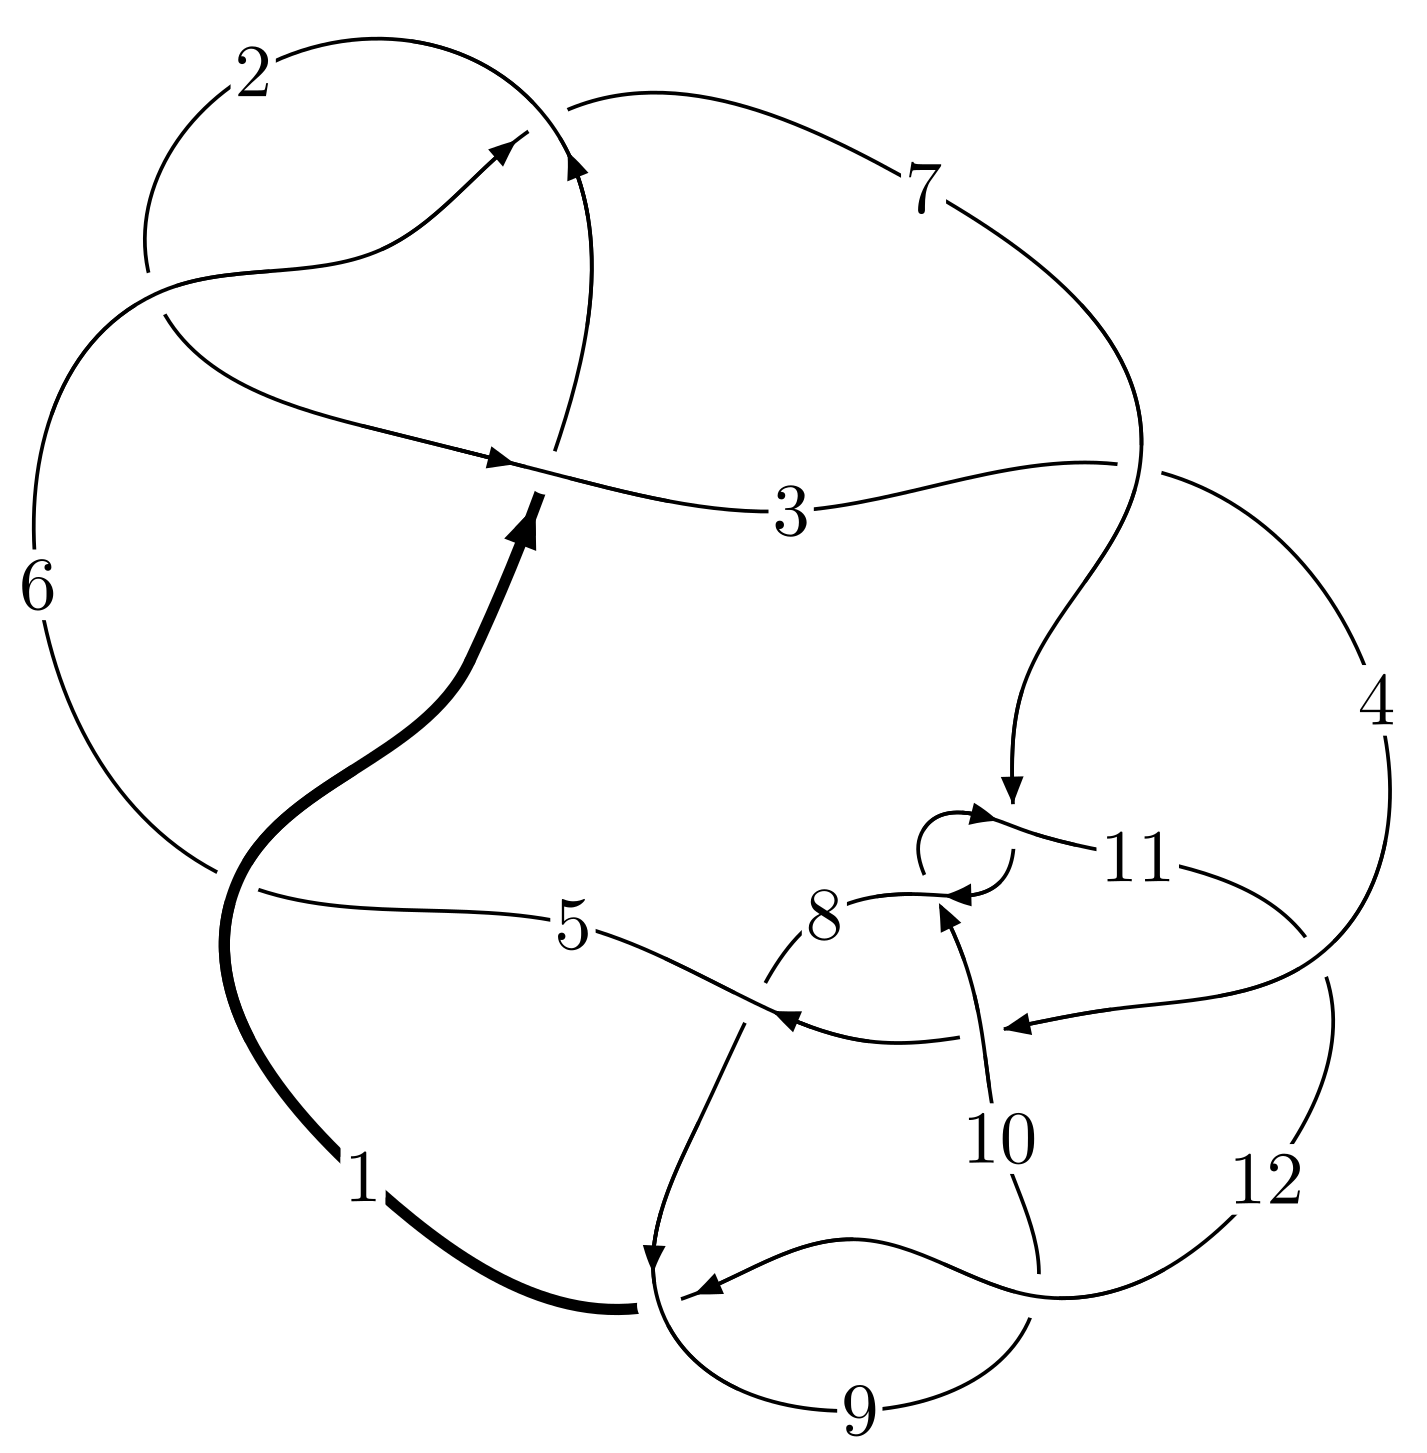
\includegraphics[width=112pt]{../../../GIT/diagram.site/Diagrams/png/1061_12a_0260.png}\\
\ \ \ A knot diagram\footnotemark}&
\allowdisplaybreaks
\textbf{Linearized knot diagam} \\
\cline{2-2}
 &
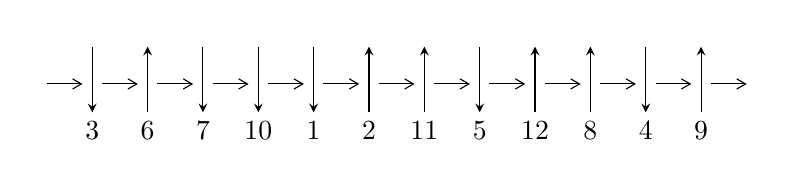
\begin{tikzpicture}[x=20pt, y=17pt]
	% nodes
	\node (C0) at (0, 0) {};
	\node (C1) at (1, 0) {};
	\node (C1U) at (1, +1) {};
	\node (C1D) at (1, -1) {3};

	\node (C2) at (2, 0) {};
	\node (C2U) at (2, +1) {};
	\node (C2D) at (2, -1) {6};

	\node (C3) at (3, 0) {};
	\node (C3U) at (3, +1) {};
	\node (C3D) at (3, -1) {7};

	\node (C4) at (4, 0) {};
	\node (C4U) at (4, +1) {};
	\node (C4D) at (4, -1) {10};

	\node (C5) at (5, 0) {};
	\node (C5U) at (5, +1) {};
	\node (C5D) at (5, -1) {1};

	\node (C6) at (6, 0) {};
	\node (C6U) at (6, +1) {};
	\node (C6D) at (6, -1) {2};

	\node (C7) at (7, 0) {};
	\node (C7U) at (7, +1) {};
	\node (C7D) at (7, -1) {11};

	\node (C8) at (8, 0) {};
	\node (C8U) at (8, +1) {};
	\node (C8D) at (8, -1) {5};

	\node (C9) at (9, 0) {};
	\node (C9U) at (9, +1) {};
	\node (C9D) at (9, -1) {12};

	\node (C10) at (10, 0) {};
	\node (C10U) at (10, +1) {};
	\node (C10D) at (10, -1) {8};

	\node (C11) at (11, 0) {};
	\node (C11U) at (11, +1) {};
	\node (C11D) at (11, -1) {4};

	\node (C12) at (12, 0) {};
	\node (C12U) at (12, +1) {};
	\node (C12D) at (12, -1) {9};
	\node (C13) at (13, 0) {};

	% arrows
	\draw[->,>={angle 60}]
	(C0) edge (C1) (C1) edge (C2) (C2) edge (C3) (C3) edge (C4) (C4) edge (C5) (C5) edge (C6) (C6) edge (C7) (C7) edge (C8) (C8) edge (C9) (C9) edge (C10) (C10) edge (C11) (C11) edge (C12) (C12) edge (C13) ;	\draw[->,>=stealth]
	(C1U) edge (C1D) (C2D) edge (C2U) (C3U) edge (C3D) (C4U) edge (C4D) (C5U) edge (C5D) (C6D) edge (C6U) (C7D) edge (C7U) (C8U) edge (C8D) (C9D) edge (C9U) (C10D) edge (C10U) (C11U) edge (C11D) (C12D) edge (C12U) ;
	\end{tikzpicture} \\
\hhline{~~} \\& 
\textbf{Solving Sequence} \\ \cline{2-2} 
 &
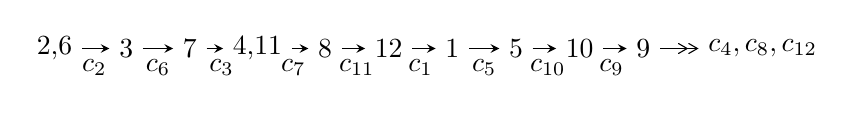
\begin{tikzpicture}[x=23pt, y=7pt]
	% node
	\node (A0) at (-1/8, 0) {2,6};
	\node (A1) at (1, 0) {3};
	\node (A2) at (2, 0) {7};
	\node (A3) at (49/16, 0) {4,11};
	\node (A4) at (33/8, 0) {8};
	\node (A5) at (41/8, 0) {12};
	\node (A6) at (49/8, 0) {1};
	\node (A7) at (57/8, 0) {5};
	\node (A8) at (65/8, 0) {10};
	\node (A9) at (73/8, 0) {9};
	\node (C1) at (1/2, -1) {$c_{2}$};
	\node (C2) at (3/2, -1) {$c_{6}$};
	\node (C3) at (5/2, -1) {$c_{3}$};
	\node (C4) at (29/8, -1) {$c_{7}$};
	\node (C5) at (37/8, -1) {$c_{11}$};
	\node (C6) at (45/8, -1) {$c_{1}$};
	\node (C7) at (53/8, -1) {$c_{5}$};
	\node (C8) at (61/8, -1) {$c_{10}$};
	\node (C9) at (69/8, -1) {$c_{9}$};
	\node (A10) at (11, 0) {$c_{4},c_{8},c_{12}$};

	% edge
	\draw[->,>=stealth]	
	(A0) edge (A1) (A1) edge (A2) (A2) edge (A3) (A3) edge (A4) (A4) edge (A5) (A5) edge (A6) (A6) edge (A7) (A7) edge (A8) (A8) edge (A9) ;
	\draw[->>,>={angle 60}]	
	(A9) edge (A10);
\end{tikzpicture} \\ 

\end{tabular} \\

\footnotetext{
The image of knot diagram is generated by the software ``\textbf{Draw programme}" developed by Andrew Bartholomew(\url{http://www.layer8.co.uk/maths/draw/index.htm\#Running-draw}), where we modified some parts for our purpose(\url{https://github.com/CATsTAILs/LinksPainter}).
}\phantom \\ \newline 
\centering \textbf{Ideals for irreducible components\footnotemark of $X_{\text{par}}$} 
 
\begin{align*}
I^u_{1}&=\langle 
-1.75234\times10^{17} u^{39}+5.61074\times10^{17} u^{38}+\cdots+1.58801\times10^{18} b-1.77103\times10^{18},\\
\phantom{I^u_{1}}&\phantom{= \langle  }-9.73786\times10^{17} u^{39}-2.24750\times10^{17} u^{38}+\cdots+3.17601\times10^{18} a+6.50880\times10^{18},\\
\phantom{I^u_{1}}&\phantom{= \langle  }u^{40}+2 u^{39}+\cdots-15 u-4\rangle \\
I^u_{2}&=\langle 
142 u^{29} a+u^{29}+\cdots-811 a+77,\;4 u^{28} a+u^{29}+\cdots-5 a+16,\;u^{30}+u^{29}+\cdots+u-1\rangle \\
I^u_{3}&=\langle 
2 u^4-2 u^3+2 u^2+2 b- u,\;-2 u^2+2 a+u-2,\;u^5- u^4+2 u^3- u^2+u-1\rangle \\
I^u_{4}&=\langle 
- a u+b-2 a+u+1,\;a^2-2 a+2,\;u^2+u+1\rangle \\
\\
\end{align*}
\raggedright * 4 irreducible components of $\dim_{\mathbb{C}}=0$, with total 109 representations.\\
\footnotetext{All coefficients of polynomials are rational numbers. But the coefficients are sometimes approximated in decimal forms when there is not enough margin.}
\newpage
\renewcommand{\arraystretch}{1}
\centering \section*{I. $I^u_{1}= \langle -1.75\times10^{17} u^{39}+5.61\times10^{17} u^{38}+\cdots+1.59\times10^{18} b-1.77\times10^{18},\;-9.74\times10^{17} u^{39}-2.25\times10^{17} u^{38}+\cdots+3.18\times10^{18} a+6.51\times10^{18},\;u^{40}+2 u^{39}+\cdots-15 u-4 \rangle$}
\flushleft \textbf{(i) Arc colorings}\\
\begin{tabular}{m{7pt} m{180pt} m{7pt} m{180pt} }
\flushright $a_{2}=$&$\begin{pmatrix}1\\0\end{pmatrix}$ \\
\flushright $a_{6}=$&$\begin{pmatrix}0\\u\end{pmatrix}$ \\
\flushright $a_{3}=$&$\begin{pmatrix}1\\- u^2\end{pmatrix}$ \\
\flushright $a_{7}=$&$\begin{pmatrix}u\\u\end{pmatrix}$ \\
\flushright $a_{4}=$&$\begin{pmatrix}u^4+u^2+1\\u^4\end{pmatrix}$ \\
\flushright $a_{11}=$&$\begin{pmatrix}0.306607 u^{39}+0.0707647 u^{38}+\cdots-2.18335 u-2.04936\\0.110349 u^{39}-0.353320 u^{38}+\cdots+4.43538 u+1.11525\end{pmatrix}$ \\
\flushright $a_{8}=$&$\begin{pmatrix}0.330016 u^{39}+0.209936 u^{38}+\cdots-2.54790 u-1.41013\\0.167912 u^{39}-0.146809 u^{38}+\cdots+3.63862 u+0.864836\end{pmatrix}$ \\
\flushright $a_{12}=$&$\begin{pmatrix}0.233887 u^{39}+0.0964315 u^{38}+\cdots-2.14298 u-1.71555\\0.223896 u^{39}+0.0820644 u^{38}+\cdots+1.09448 u+0.165309\end{pmatrix}$ \\
\flushright $a_{1}=$&$\begin{pmatrix}u^2+1\\- u^4\end{pmatrix}$ \\
\flushright $a_{5}=$&$\begin{pmatrix}u^5+2 u^3+u\\- u^7- u^5+u\end{pmatrix}$ \\
\flushright $a_{10}=$&$\begin{pmatrix}0.606364 u^{39}+0.274704 u^{38}+\cdots-4.91727 u-2.84677\\0.385943 u^{39}-0.202353 u^{38}+\cdots+5.39621 u+1.32664\end{pmatrix}$ \\
\flushright $a_{9}=$&$\begin{pmatrix}0.263635 u^{39}+0.0269093 u^{38}+\cdots-1.67340 u-1.47960\\0.148444 u^{39}-0.225204 u^{38}+\cdots+3.90113 u+0.775015\end{pmatrix}$\\&\end{tabular}
\flushleft \textbf{(ii) Obstruction class $= -1$}\\~\\
\flushleft \textbf{(iii) Cusp Shapes $= -\frac{1027807058031671441}{794003375424954487} u^{39}-\frac{7796249979768242351}{3176013501699817948} u^{38}+\cdots-\frac{1978648037828171537}{794003375424954487} u+\frac{67049658634384246}{794003375424954487}$}\\~\\
\newpage\renewcommand{\arraystretch}{1}
\flushleft \textbf{(iv) u-Polynomials at the component}\newline \\
\begin{tabular}{m{50pt}|m{274pt}}
Crossings & \hspace{64pt}u-Polynomials at each crossing \\
\hline $$\begin{aligned}c_{1}\end{aligned}$$&$\begin{aligned}
&u^{40}+22 u^{39}+\cdots- u+16
\end{aligned}$\\
\hline $$\begin{aligned}c_{2},c_{6}\end{aligned}$$&$\begin{aligned}
&u^{40}-2 u^{39}+\cdots+15 u-4
\end{aligned}$\\
\hline $$\begin{aligned}c_{3},c_{5}\end{aligned}$$&$\begin{aligned}
&u^{40}+2 u^{39}+\cdots+871 u-676
\end{aligned}$\\
\hline $$\begin{aligned}c_{4}\end{aligned}$$&$\begin{aligned}
&u^{40}-3 u^{39}+\cdots+512 u+2048
\end{aligned}$\\
\hline $$\begin{aligned}c_{7},c_{9},c_{10}\\c_{12}\end{aligned}$$&$\begin{aligned}
&u^{40}-5 u^{39}+\cdots-3 u-1
\end{aligned}$\\
\hline $$\begin{aligned}c_{8},c_{11}\end{aligned}$$&$\begin{aligned}
&32(32 u^{40}+48 u^{39}+\cdots+8 u+4)
\end{aligned}$\\
\hline
\end{tabular}\\~\\
\newpage\renewcommand{\arraystretch}{1}
\flushleft \textbf{(v) Riley Polynomials at the component}\newline \\
\begin{tabular}{m{50pt}|m{274pt}}
Crossings & \hspace{64pt}Riley Polynomials at each crossing \\
\hline $$\begin{aligned}c_{1}\end{aligned}$$&$\begin{aligned}
&y^{40}-6 y^{39}+\cdots-3905 y+256
\end{aligned}$\\
\hline $$\begin{aligned}c_{2},c_{6}\end{aligned}$$&$\begin{aligned}
&y^{40}+22 y^{39}+\cdots- y+16
\end{aligned}$\\
\hline $$\begin{aligned}c_{3},c_{5}\end{aligned}$$&$\begin{aligned}
&y^{40}-34 y^{39}+\cdots+2269839 y+456976
\end{aligned}$\\
\hline $$\begin{aligned}c_{4}\end{aligned}$$&$\begin{aligned}
&y^{40}-13 y^{39}+\cdots-63176704 y+4194304
\end{aligned}$\\
\hline $$\begin{aligned}c_{7},c_{9},c_{10}\\c_{12}\end{aligned}$$&$\begin{aligned}
&y^{40}+27 y^{39}+\cdots+25 y+1
\end{aligned}$\\
\hline $$\begin{aligned}c_{8},c_{11}\end{aligned}$$&$\begin{aligned}
&1024(1024 y^{40}-27904 y^{39}+\cdots+16 y+16)
\end{aligned}$\\
\hline
\end{tabular}\\~\\
\newpage\flushleft \textbf{(vi) Complex Volumes and Cusp Shapes}
$$\begin{array}{c|c|c}  
\text{Solutions to }I^u_{1}& \I (\text{vol} + \sqrt{-1}CS) & \text{Cusp shape}\\
 \hline 
\begin{aligned}
u &= -0.748783 + 0.635787 I \\
a &= \phantom{-}0.497441 - 0.487921 I \\
b &= -0.443502 + 0.321931 I\end{aligned}
 & -3.86456 - 4.42335 I & -6.59807 + 7.34601 I \\ \hline\begin{aligned}
u &= -0.748783 - 0.635787 I \\
a &= \phantom{-}0.497441 + 0.487921 I \\
b &= -0.443502 - 0.321931 I\end{aligned}
 & -3.86456 + 4.42335 I & -6.59807 - 7.34601 I \\ \hline\begin{aligned}
u &= \phantom{-}0.370444 + 0.884043 I \\
a &= -0.741241 - 0.879542 I \\
b &= -0.990076 + 0.305719 I\end{aligned}
 & \phantom{-}1.27740 + 1.88898 I & -6.0015 - 15.6995 I \\ \hline\begin{aligned}
u &= \phantom{-}0.370444 - 0.884043 I \\
a &= -0.741241 + 0.879542 I \\
b &= -0.990076 - 0.305719 I\end{aligned}
 & \phantom{-}1.27740 - 1.88898 I & -6.0015 + 15.6995 I \\ \hline\begin{aligned}
u &= \phantom{-}0.936692 + 0.132944 I \\
a &= -0.36069 - 2.07229 I \\
b &= -0.283700 - 0.679214 I\end{aligned}
 & -10.28620 - 2.94658 I & -8.50665 + 2.50672 I \\ \hline\begin{aligned}
u &= \phantom{-}0.936692 - 0.132944 I \\
a &= -0.36069 + 2.07229 I \\
b &= -0.283700 + 0.679214 I\end{aligned}
 & -10.28620 + 2.94658 I & -8.50665 - 2.50672 I \\ \hline\begin{aligned}
u &= -0.893287 + 0.111704 I \\
a &= -0.24516 + 2.54481 I \\
b &= -0.611222 + 0.896510 I\end{aligned}
 & -11.6323 + 12.6478 I & -5.02011 - 6.24043 I \\ \hline\begin{aligned}
u &= -0.893287 - 0.111704 I \\
a &= -0.24516 - 2.54481 I \\
b &= -0.611222 - 0.896510 I\end{aligned}
 & -11.6323 - 12.6478 I & -5.02011 + 6.24043 I \\ \hline\begin{aligned}
u &= -0.433282 + 1.016950 I \\
a &= -0.826445 + 0.289312 I \\
b &= -1.227630 + 0.661551 I\end{aligned}
 & -1.48385 - 1.77946 I & -1.213579 + 0.177328 I \\ \hline\begin{aligned}
u &= -0.433282 - 1.016950 I \\
a &= -0.826445 - 0.289312 I \\
b &= -1.227630 - 0.661551 I\end{aligned}
 & -1.48385 + 1.77946 I & -1.213579 - 0.177328 I\\
 \hline 
 \end{array}$$\newpage$$\begin{array}{c|c|c}  
\text{Solutions to }I^u_{1}& \I (\text{vol} + \sqrt{-1}CS) & \text{Cusp shape}\\
 \hline 
\begin{aligned}
u &= \phantom{-}0.735196 + 0.474957 I \\
a &= \phantom{-}0.73676 + 1.52515 I \\
b &= \phantom{-}0.299735 + 0.089122 I\end{aligned}
 & -4.66772 - 7.25009 I & -3.73082 + 5.45853 I \\ \hline\begin{aligned}
u &= \phantom{-}0.735196 - 0.474957 I \\
a &= \phantom{-}0.73676 - 1.52515 I \\
b &= \phantom{-}0.299735 - 0.089122 I\end{aligned}
 & -4.66772 + 7.25009 I & -3.73082 - 5.45853 I \\ \hline\begin{aligned}
u &= \phantom{-}0.590773 + 1.005950 I \\
a &= \phantom{-}0.968619 + 0.798321 I \\
b &= \phantom{-}2.11021 + 1.04129 I\end{aligned}
 & -6.21633 + 12.24890 I & -5.37332 - 9.94766 I \\ \hline\begin{aligned}
u &= \phantom{-}0.590773 - 1.005950 I \\
a &= \phantom{-}0.968619 - 0.798321 I \\
b &= \phantom{-}2.11021 - 1.04129 I\end{aligned}
 & -6.21633 - 12.24890 I & -5.37332 + 9.94766 I \\ \hline\begin{aligned}
u &= -0.691554 + 0.944218 I \\
a &= \phantom{-}0.219338 - 0.024885 I \\
b &= \phantom{-}0.996837 - 0.702945 I\end{aligned}
 & -4.74262 - 0.98558 I & -10.53556 - 1.39688 I \\ \hline\begin{aligned}
u &= -0.691554 - 0.944218 I \\
a &= \phantom{-}0.219338 + 0.024885 I \\
b &= \phantom{-}0.996837 + 0.702945 I\end{aligned}
 & -4.74262 + 0.98558 I & -10.53556 + 1.39688 I \\ \hline\begin{aligned}
u &= -0.429290 + 1.094810 I \\
a &= \phantom{-}1.52361 + 0.07658 I \\
b &= \phantom{-}2.25201 + 0.30626 I\end{aligned}
 & -1.51361 - 4.99339 I & -1.46170 + 7.63475 I \\ \hline\begin{aligned}
u &= -0.429290 - 1.094810 I \\
a &= \phantom{-}1.52361 - 0.07658 I \\
b &= \phantom{-}2.25201 - 0.30626 I\end{aligned}
 & -1.51361 + 4.99339 I & -1.46170 - 7.63475 I \\ \hline\begin{aligned}
u &= -0.810513\phantom{ +0.000000I} \\
a &= -1.68768\phantom{ +0.000000I} \\
b &= \phantom{-}0.0637912\phantom{ +0.000000I}\end{aligned}
 & -1.48600\phantom{ +0.000000I} & -8.82010\phantom{ +0.000000I} \\ \hline\begin{aligned}
u &= -0.298599 + 0.749021 I \\
a &= -0.230770 + 0.654861 I \\
b &= -0.010961 + 0.514630 I\end{aligned}
 & -0.340785 - 1.228130 I & -3.72246 + 5.05532 I\\
 \hline 
 \end{array}$$\newpage$$\begin{array}{c|c|c}  
\text{Solutions to }I^u_{1}& \I (\text{vol} + \sqrt{-1}CS) & \text{Cusp shape}\\
 \hline 
\begin{aligned}
u &= -0.298599 - 0.749021 I \\
a &= -0.230770 - 0.654861 I \\
b &= -0.010961 - 0.514630 I\end{aligned}
 & -0.340785 + 1.228130 I & -3.72246 - 5.05532 I \\ \hline\begin{aligned}
u &= \phantom{-}0.043335 + 1.221830 I \\
a &= -1.41988 + 0.07791 I \\
b &= -2.52419 - 0.17469 I\end{aligned}
 & -10.36550 - 5.41067 I & -11.07269 + 4.06686 I \\ \hline\begin{aligned}
u &= \phantom{-}0.043335 - 1.221830 I \\
a &= -1.41988 - 0.07791 I \\
b &= -2.52419 + 0.17469 I\end{aligned}
 & -10.36550 + 5.41067 I & -11.07269 - 4.06686 I \\ \hline\begin{aligned}
u &= \phantom{-}0.340574 + 0.682840 I \\
a &= -0.201912 - 1.203320 I \\
b &= -1.136840 - 0.348081 I\end{aligned}
 & \phantom{-}1.86966 + 1.36297 I & \phantom{-}7.37182 + 2.84076 I \\ \hline\begin{aligned}
u &= \phantom{-}0.340574 - 0.682840 I \\
a &= -0.201912 + 1.203320 I \\
b &= -1.136840 + 0.348081 I\end{aligned}
 & \phantom{-}1.86966 - 1.36297 I & \phantom{-}7.37182 - 2.84076 I \\ \hline\begin{aligned}
u &= \phantom{-}0.732733\phantom{ +0.000000I} \\
a &= \phantom{-}0.0215748\phantom{ +0.000000I} \\
b &= \phantom{-}0.419703\phantom{ +0.000000I}\end{aligned}
 & -1.91322\phantom{ +0.000000I} & -6.72230\phantom{ +0.000000I} \\ \hline\begin{aligned}
u &= \phantom{-}0.455122 + 1.187290 I \\
a &= \phantom{-}0.297888 + 0.394001 I \\
b &= \phantom{-}0.358967 + 0.124690 I\end{aligned}
 & -5.28776 + 4.30879 I & -10.28965 - 3.19866 I \\ \hline\begin{aligned}
u &= \phantom{-}0.455122 - 1.187290 I \\
a &= \phantom{-}0.297888 - 0.394001 I \\
b &= \phantom{-}0.358967 - 0.124690 I\end{aligned}
 & -5.28776 - 4.30879 I & -10.28965 + 3.19866 I \\ \hline\begin{aligned}
u &= -0.459206 + 1.219680 I \\
a &= \phantom{-}0.496160 + 0.913959 I \\
b &= \phantom{-}0.85669 + 1.97796 I\end{aligned}
 & -5.08353 - 4.54254 I & -11.30086 + 4.03212 I \\ \hline\begin{aligned}
u &= -0.459206 - 1.219680 I \\
a &= \phantom{-}0.496160 - 0.913959 I \\
b &= \phantom{-}0.85669 - 1.97796 I\end{aligned}
 & -5.08353 + 4.54254 I & -11.30086 - 4.03212 I\\
 \hline 
 \end{array}$$\newpage$$\begin{array}{c|c|c}  
\text{Solutions to }I^u_{1}& \I (\text{vol} + \sqrt{-1}CS) & \text{Cusp shape}\\
 \hline 
\begin{aligned}
u &= -0.395526 + 1.274220 I \\
a &= \phantom{-}1.88050 + 0.61513 I \\
b &= \phantom{-}2.81622 - 0.05833 I\end{aligned}
 & -15.9475 + 8.1867 I & -9.06394 - 3.34621 I \\ \hline\begin{aligned}
u &= -0.395526 - 1.274220 I \\
a &= \phantom{-}1.88050 - 0.61513 I \\
b &= \phantom{-}2.81622 + 0.05833 I\end{aligned}
 & -15.9475 - 8.1867 I & -9.06394 + 3.34621 I \\ \hline\begin{aligned}
u &= -0.521628 + 1.236120 I \\
a &= -2.58052 + 0.56454 I \\
b &= -3.72507 + 0.61373 I\end{aligned}
 & -15.0274 - 17.7587 I & -7.82233 + 9.25326 I \\ \hline\begin{aligned}
u &= -0.521628 - 1.236120 I \\
a &= -2.58052 - 0.56454 I \\
b &= -3.72507 - 0.61373 I\end{aligned}
 & -15.0274 + 17.7587 I & -7.82233 - 9.25326 I \\ \hline\begin{aligned}
u &= \phantom{-}0.380735 + 1.301160 I \\
a &= \phantom{-}1.75721 - 0.48165 I \\
b &= \phantom{-}2.71281 - 0.14779 I\end{aligned}
 & -14.8538 + 1.6038 I & -12.02430 - 0.97260 I \\ \hline\begin{aligned}
u &= \phantom{-}0.380735 - 1.301160 I \\
a &= \phantom{-}1.75721 + 0.48165 I \\
b &= \phantom{-}2.71281 + 0.14779 I\end{aligned}
 & -14.8538 - 1.6038 I & -12.02430 + 0.97260 I \\ \hline\begin{aligned}
u &= \phantom{-}0.538772 + 1.252000 I \\
a &= -1.97956 - 0.36072 I \\
b &= -2.92363 - 0.63492 I\end{aligned}
 & -13.7050 + 8.2667 I & -10.58240 - 5.91047 I \\ \hline\begin{aligned}
u &= \phantom{-}0.538772 - 1.252000 I \\
a &= -1.97956 + 0.36072 I \\
b &= -2.92363 + 0.63492 I\end{aligned}
 & -13.7050 - 8.2667 I & -10.58240 + 5.91047 I \\ \hline\begin{aligned}
u &= -0.481597 + 0.152677 I \\
a &= -0.83330 - 1.69163 I \\
b &= -0.018409 - 0.472499 I\end{aligned}
 & \phantom{-}1.02330 + 1.25064 I & \phantom{-}5.09440 - 3.99293 I \\ \hline\begin{aligned}
u &= -0.481597 - 0.152677 I \\
a &= -0.83330 + 1.69163 I \\
b &= -0.018409 + 0.472499 I\end{aligned}
 & \phantom{-}1.02330 - 1.25064 I & \phantom{-}5.09440 + 3.99293 I\\
 \hline 
 \end{array}$$\newpage\newpage\renewcommand{\arraystretch}{1}
\centering \section*{II. $I^u_{2}= \langle 142 u^{29} a+u^{29}+\cdots-811 a+77,\;4 u^{28} a+u^{29}+\cdots-5 a+16,\;u^{30}+u^{29}+\cdots+u-1 \rangle$}
\flushleft \textbf{(i) Arc colorings}\\
\begin{tabular}{m{7pt} m{180pt} m{7pt} m{180pt} }
\flushright $a_{2}=$&$\begin{pmatrix}1\\0\end{pmatrix}$ \\
\flushright $a_{6}=$&$\begin{pmatrix}0\\u\end{pmatrix}$ \\
\flushright $a_{3}=$&$\begin{pmatrix}1\\- u^2\end{pmatrix}$ \\
\flushright $a_{7}=$&$\begin{pmatrix}u\\u\end{pmatrix}$ \\
\flushright $a_{4}=$&$\begin{pmatrix}u^4+u^2+1\\u^4\end{pmatrix}$ \\
\flushright $a_{11}=$&$\begin{pmatrix}a\\-0.181354 a u^{29}-0.00127714 u^{29}+\cdots+1.03576 a-0.0983397\end{pmatrix}$ \\
\flushright $a_{8}=$&$\begin{pmatrix}1.07791 a u^{29}-1.96424 u^{29}+\cdots-0.00127714 a+2.75351\\1.96424 a u^{29}-1.90166 u^{29}+\cdots+0.246488 a+3.57216\end{pmatrix}$ \\
\flushright $a_{12}=$&$\begin{pmatrix}0.494253 a u^{29}-0.609195 u^{29}+\cdots+0.0574713 a+0.0919540\\0.132822 a u^{29}-0.365262 u^{29}+\cdots+0.227331 a+0.874840\end{pmatrix}$ \\
\flushright $a_{1}=$&$\begin{pmatrix}u^2+1\\- u^4\end{pmatrix}$ \\
\flushright $a_{5}=$&$\begin{pmatrix}u^5+2 u^3+u\\- u^7- u^5+u\end{pmatrix}$ \\
\flushright $a_{10}=$&$\begin{pmatrix}u^{29}+8 u^{27}+\cdots+4 u^3+u\\u^{29}+7 u^{27}+\cdots- u^3- u\end{pmatrix}$ \\
\flushright $a_{9}=$&$\begin{pmatrix}1.03576 a u^{29}-2.09834 u^{29}+\cdots-0.246488 a+1.42784\\0.937420 a u^{29}+0.922095 u^{29}+\cdots+0.181354 a+2.00128\end{pmatrix}$\\&\end{tabular}
\flushleft \textbf{(ii) Obstruction class $= -1$}\\~\\
\flushleft \textbf{(iii) Cusp Shapes $= -4 u^{29}-4 u^{28}-32 u^{27}-28 u^{26}-120 u^{25}-96 u^{24}-260 u^{23}-196 u^{22}-332 u^{21}-256 u^{20}-196 u^{19}-204 u^{18}+76 u^{17}-72 u^{16}+224 u^{15}+52 u^{14}+136 u^{13}+108 u^{12}-12 u^{11}+100 u^{10}-60 u^9+44 u^8-32 u^7-12 u^6-8 u^5-24 u^4+8 u^3-12 u^2+8 u-6$}\\~\\
\newpage\renewcommand{\arraystretch}{1}
\flushleft \textbf{(iv) u-Polynomials at the component}\newline \\
\begin{tabular}{m{50pt}|m{274pt}}
Crossings & \hspace{64pt}u-Polynomials at each crossing \\
\hline $$\begin{aligned}c_{1}\end{aligned}$$&$\begin{aligned}
&(u^{30}+17 u^{29}+\cdots- u+1)^{2}
\end{aligned}$\\
\hline $$\begin{aligned}c_{2},c_{6}\end{aligned}$$&$\begin{aligned}
&(u^{30}- u^{29}+\cdots- u-1)^{2}
\end{aligned}$\\
\hline $$\begin{aligned}c_{3},c_{5}\end{aligned}$$&$\begin{aligned}
&(u^{30}+u^{29}+\cdots+7 u-1)^{2}
\end{aligned}$\\
\hline $$\begin{aligned}c_{4}\end{aligned}$$&$\begin{aligned}
&(u^{30}+u^{29}+\cdots+u-1)^{2}
\end{aligned}$\\
\hline $$\begin{aligned}c_{7},c_{9},c_{10}\\c_{12}\end{aligned}$$&$\begin{aligned}
&u^{60}+11 u^{59}+\cdots+20 u+1
\end{aligned}$\\
\hline $$\begin{aligned}c_{8},c_{11}\end{aligned}$$&$\begin{aligned}
&u^{60}+5 u^{59}+\cdots-23472726 u+8156149
\end{aligned}$\\
\hline
\end{tabular}\\~\\
\newpage\renewcommand{\arraystretch}{1}
\flushleft \textbf{(v) Riley Polynomials at the component}\newline \\
\begin{tabular}{m{50pt}|m{274pt}}
Crossings & \hspace{64pt}Riley Polynomials at each crossing \\
\hline $$\begin{aligned}c_{1}\end{aligned}$$&$\begin{aligned}
&(y^{30}-7 y^{29}+\cdots-25 y+1)^{2}
\end{aligned}$\\
\hline $$\begin{aligned}c_{2},c_{6}\end{aligned}$$&$\begin{aligned}
&(y^{30}+17 y^{29}+\cdots- y+1)^{2}
\end{aligned}$\\
\hline $$\begin{aligned}c_{3},c_{5}\end{aligned}$$&$\begin{aligned}
&(y^{30}-31 y^{29}+\cdots-49 y+1)^{2}
\end{aligned}$\\
\hline $$\begin{aligned}c_{4}\end{aligned}$$&$\begin{aligned}
&(y^{30}-11 y^{29}+\cdots- y+1)^{2}
\end{aligned}$\\
\hline $$\begin{aligned}c_{7},c_{9},c_{10}\\c_{12}\end{aligned}$$&$\begin{aligned}
&y^{60}+43 y^{59}+\cdots+64 y+1
\end{aligned}$\\
\hline $$\begin{aligned}c_{8},c_{11}\end{aligned}$$&$\begin{aligned}
&y^{60}-37 y^{59}+\cdots-1403816325059308 y+66522766510201
\end{aligned}$\\
\hline
\end{tabular}\\~\\
\newpage\flushleft \textbf{(vi) Complex Volumes and Cusp Shapes}
$$\begin{array}{c|c|c}  
\text{Solutions to }I^u_{2}& \I (\text{vol} + \sqrt{-1}CS) & \text{Cusp shape}\\
 \hline 
\begin{aligned}
u &= \phantom{-}0.095027 + 1.028250 I \\
a &= \phantom{-}1.034680 + 0.226441 I \\
b &= \phantom{-}2.30549 + 0.52767 I\end{aligned}
 & -5.04140 - 2.04857 I & -7.94351 + 2.92796 I \\ \hline\begin{aligned}
u &= \phantom{-}0.095027 + 1.028250 I \\
a &= \phantom{-}0.716670 + 0.339240 I \\
b &= \phantom{-}0.426153 - 0.394651 I\end{aligned}
 & -5.04140 - 2.04857 I & -7.94351 + 2.92796 I \\ \hline\begin{aligned}
u &= \phantom{-}0.095027 - 1.028250 I \\
a &= \phantom{-}1.034680 - 0.226441 I \\
b &= \phantom{-}2.30549 - 0.52767 I\end{aligned}
 & -5.04140 + 2.04857 I & -7.94351 - 2.92796 I \\ \hline\begin{aligned}
u &= \phantom{-}0.095027 - 1.028250 I \\
a &= \phantom{-}0.716670 - 0.339240 I \\
b &= \phantom{-}0.426153 + 0.394651 I\end{aligned}
 & -5.04140 + 2.04857 I & -7.94351 - 2.92796 I \\ \hline\begin{aligned}
u &= -0.486868 + 0.916512 I \\
a &= -0.940915 - 0.299954 I \\
b &= -1.039270 - 0.311684 I\end{aligned}
 & -1.61342 - 2.06909 I & -0.15841 + 3.38718 I \\ \hline\begin{aligned}
u &= -0.486868 + 0.916512 I \\
a &= -0.447231 + 0.917418 I \\
b &= -1.24616 + 1.37787 I\end{aligned}
 & -1.61342 - 2.06909 I & -0.15841 + 3.38718 I \\ \hline\begin{aligned}
u &= -0.486868 - 0.916512 I \\
a &= -0.940915 + 0.299954 I \\
b &= -1.039270 + 0.311684 I\end{aligned}
 & -1.61342 + 2.06909 I & -0.15841 - 3.38718 I \\ \hline\begin{aligned}
u &= -0.486868 - 0.916512 I \\
a &= -0.447231 - 0.917418 I \\
b &= -1.24616 - 1.37787 I\end{aligned}
 & -1.61342 + 2.06909 I & -0.15841 - 3.38718 I \\ \hline\begin{aligned}
u &= \phantom{-}0.336716 + 1.031390 I \\
a &= -0.398995 + 0.561283 I \\
b &= -1.50734 - 0.06821 I\end{aligned}
 & -6.92657 + 2.97945 I & -9.92079 - 5.34085 I \\ \hline\begin{aligned}
u &= \phantom{-}0.336716 + 1.031390 I \\
a &= \phantom{-}0.64157 + 1.48251 I \\
b &= \phantom{-}1.74824 + 1.30378 I\end{aligned}
 & -6.92657 + 2.97945 I & -9.92079 - 5.34085 I\\
 \hline 
 \end{array}$$\newpage$$\begin{array}{c|c|c}  
\text{Solutions to }I^u_{2}& \I (\text{vol} + \sqrt{-1}CS) & \text{Cusp shape}\\
 \hline 
\begin{aligned}
u &= \phantom{-}0.336716 - 1.031390 I \\
a &= -0.398995 - 0.561283 I \\
b &= -1.50734 + 0.06821 I\end{aligned}
 & -6.92657 - 2.97945 I & -9.92079 + 5.34085 I \\ \hline\begin{aligned}
u &= \phantom{-}0.336716 - 1.031390 I \\
a &= \phantom{-}0.64157 - 1.48251 I \\
b &= \phantom{-}1.74824 - 1.30378 I\end{aligned}
 & -6.92657 - 2.97945 I & -9.92079 + 5.34085 I \\ \hline\begin{aligned}
u &= \phantom{-}0.500817 + 0.966472 I \\
a &= \phantom{-}0.522463 + 0.779303 I \\
b &= \phantom{-}0.877769 + 0.011516 I\end{aligned}
 & -2.27531 + 7.42449 I & -2.02063 - 8.82247 I \\ \hline\begin{aligned}
u &= \phantom{-}0.500817 + 0.966472 I \\
a &= -0.759314 - 1.014940 I \\
b &= -1.98900 - 1.15324 I\end{aligned}
 & -2.27531 + 7.42449 I & -2.02063 - 8.82247 I \\ \hline\begin{aligned}
u &= \phantom{-}0.500817 - 0.966472 I \\
a &= \phantom{-}0.522463 - 0.779303 I \\
b &= \phantom{-}0.877769 - 0.011516 I\end{aligned}
 & -2.27531 - 7.42449 I & -2.02063 + 8.82247 I \\ \hline\begin{aligned}
u &= \phantom{-}0.500817 - 0.966472 I \\
a &= -0.759314 + 1.014940 I \\
b &= -1.98900 + 1.15324 I\end{aligned}
 & -2.27531 - 7.42449 I & -2.02063 + 8.82247 I \\ \hline\begin{aligned}
u &= -0.272716 + 0.834978 I \\
a &= \phantom{-}4.75539 + 1.58121 I \\
b &= \phantom{-}5.93533 + 1.26168 I\end{aligned}
 & -3.79299 - 1.32269 I & -1.12281 + 4.79072 I \\ \hline\begin{aligned}
u &= -0.272716 + 0.834978 I \\
a &= \phantom{-}2.73856 - 4.77786 I \\
b &= \phantom{-}1.76585 - 4.35750 I\end{aligned}
 & -3.79299 - 1.32269 I & -1.12281 + 4.79072 I \\ \hline\begin{aligned}
u &= -0.272716 - 0.834978 I \\
a &= \phantom{-}4.75539 - 1.58121 I \\
b &= \phantom{-}5.93533 - 1.26168 I\end{aligned}
 & -3.79299 + 1.32269 I & -1.12281 - 4.79072 I \\ \hline\begin{aligned}
u &= -0.272716 - 0.834978 I \\
a &= \phantom{-}2.73856 + 4.77786 I \\
b &= \phantom{-}1.76585 + 4.35750 I\end{aligned}
 & -3.79299 + 1.32269 I & -1.12281 - 4.79072 I\\
 \hline 
 \end{array}$$\newpage$$\begin{array}{c|c|c}  
\text{Solutions to }I^u_{2}& \I (\text{vol} + \sqrt{-1}CS) & \text{Cusp shape}\\
 \hline 
\begin{aligned}
u &= -0.856648\phantom{ +0.000000I} \\
a &= \phantom{-}0.36456 + 2.45841 I \\
b &= -0.369614 + 0.732227 I\end{aligned}
 & -10.8641\phantom{ +0.000000I} & -7.49220\phantom{ +0.000000I} \\ \hline\begin{aligned}
u &= -0.856648\phantom{ +0.000000I} \\
a &= \phantom{-}0.36456 - 2.45841 I \\
b &= -0.369614 - 0.732227 I\end{aligned}
 & -10.8641\phantom{ +0.000000I} & -7.49220\phantom{ +0.000000I} \\ \hline\begin{aligned}
u &= -0.851057 + 0.073998 I \\
a &= \phantom{-}1.134850 + 0.440270 I \\
b &= -0.235397 + 0.177357 I\end{aligned}
 & -6.70542 + 6.72016 I & -3.40084 - 4.93754 I \\ \hline\begin{aligned}
u &= -0.851057 + 0.073998 I \\
a &= \phantom{-}0.02043 - 2.70525 I \\
b &= \phantom{-}0.471768 - 0.912252 I\end{aligned}
 & -6.70542 + 6.72016 I & -3.40084 - 4.93754 I \\ \hline\begin{aligned}
u &= -0.851057 - 0.073998 I \\
a &= \phantom{-}1.134850 - 0.440270 I \\
b &= -0.235397 - 0.177357 I\end{aligned}
 & -6.70542 - 6.72016 I & -3.40084 + 4.93754 I \\ \hline\begin{aligned}
u &= -0.851057 - 0.073998 I \\
a &= \phantom{-}0.02043 + 2.70525 I \\
b &= \phantom{-}0.471768 + 0.912252 I\end{aligned}
 & -6.70542 - 6.72016 I & -3.40084 + 4.93754 I \\ \hline\begin{aligned}
u &= \phantom{-}0.814472 + 0.061657 I \\
a &= -0.211672 - 0.026337 I \\
b &= -0.622855 + 0.448979 I\end{aligned}
 & -5.23568 - 1.35458 I & -1.234126 + 0.230757 I \\ \hline\begin{aligned}
u &= \phantom{-}0.814472 + 0.061657 I \\
a &= \phantom{-}0.71424 + 2.65174 I \\
b &= \phantom{-}0.706924 + 1.195690 I\end{aligned}
 & -5.23568 - 1.35458 I & -1.234126 + 0.230757 I \\ \hline\begin{aligned}
u &= \phantom{-}0.814472 - 0.061657 I \\
a &= -0.211672 + 0.026337 I \\
b &= -0.622855 - 0.448979 I\end{aligned}
 & -5.23568 + 1.35458 I & -1.234126 - 0.230757 I \\ \hline\begin{aligned}
u &= \phantom{-}0.814472 - 0.061657 I \\
a &= \phantom{-}0.71424 - 2.65174 I \\
b &= \phantom{-}0.706924 - 1.195690 I\end{aligned}
 & -5.23568 + 1.35458 I & -1.234126 - 0.230757 I\\
 \hline 
 \end{array}$$\newpage$$\begin{array}{c|c|c}  
\text{Solutions to }I^u_{2}& \I (\text{vol} + \sqrt{-1}CS) & \text{Cusp shape}\\
 \hline 
\begin{aligned}
u &= -0.517153 + 0.543315 I \\
a &= \phantom{-}0.374179 + 1.229410 I \\
b &= \phantom{-}0.087079 + 0.755551 I\end{aligned}
 & -0.57483 - 2.05267 I & \phantom{-}2.41797 + 3.48780 I \\ \hline\begin{aligned}
u &= -0.517153 + 0.543315 I \\
a &= -1.328260 + 0.442484 I \\
b &= -0.139959 - 0.267825 I\end{aligned}
 & -0.57483 - 2.05267 I & \phantom{-}2.41797 + 3.48780 I \\ \hline\begin{aligned}
u &= -0.517153 - 0.543315 I \\
a &= \phantom{-}0.374179 - 1.229410 I \\
b &= \phantom{-}0.087079 - 0.755551 I\end{aligned}
 & -0.57483 + 2.05267 I & \phantom{-}2.41797 - 3.48780 I \\ \hline\begin{aligned}
u &= -0.517153 - 0.543315 I \\
a &= -1.328260 - 0.442484 I \\
b &= -0.139959 + 0.267825 I\end{aligned}
 & -0.57483 + 2.05267 I & \phantom{-}2.41797 - 3.48780 I \\ \hline\begin{aligned}
u &= \phantom{-}0.552271 + 0.456360 I \\
a &= \phantom{-}0.048193 + 0.721700 I \\
b &= \phantom{-}0.879122 + 0.103276 I\end{aligned}
 & -0.86006 - 3.18388 I & \phantom{-}1.51706 + 3.33039 I \\ \hline\begin{aligned}
u &= \phantom{-}0.552271 + 0.456360 I \\
a &= -1.00716 - 1.45803 I \\
b &= -0.385363 + 0.145063 I\end{aligned}
 & -0.86006 - 3.18388 I & \phantom{-}1.51706 + 3.33039 I \\ \hline\begin{aligned}
u &= \phantom{-}0.552271 - 0.456360 I \\
a &= \phantom{-}0.048193 - 0.721700 I \\
b &= \phantom{-}0.879122 - 0.103276 I\end{aligned}
 & -0.86006 + 3.18388 I & \phantom{-}1.51706 - 3.33039 I \\ \hline\begin{aligned}
u &= \phantom{-}0.552271 - 0.456360 I \\
a &= -1.00716 + 1.45803 I \\
b &= -0.385363 - 0.145063 I\end{aligned}
 & -0.86006 + 3.18388 I & \phantom{-}1.51706 - 3.33039 I \\ \hline\begin{aligned}
u &= \phantom{-}0.429988 + 1.221650 I \\
a &= -0.770876 - 0.449946 I \\
b &= -0.527325 - 0.034027 I\end{aligned}
 & -9.03965 + 2.99724 I & -4.94829 - 3.11480 I \\ \hline\begin{aligned}
u &= \phantom{-}0.429988 + 1.221650 I \\
a &= -2.43427 + 1.26220 I \\
b &= -3.31200 + 0.90775 I\end{aligned}
 & -9.03965 + 2.99724 I & -4.94829 - 3.11480 I\\
 \hline 
 \end{array}$$\newpage$$\begin{array}{c|c|c}  
\text{Solutions to }I^u_{2}& \I (\text{vol} + \sqrt{-1}CS) & \text{Cusp shape}\\
 \hline 
\begin{aligned}
u &= \phantom{-}0.429988 - 1.221650 I \\
a &= -0.770876 + 0.449946 I \\
b &= -0.527325 + 0.034027 I\end{aligned}
 & -9.03965 - 2.99724 I & -4.94829 + 3.11480 I \\ \hline\begin{aligned}
u &= \phantom{-}0.429988 - 1.221650 I \\
a &= -2.43427 - 1.26220 I \\
b &= -3.31200 - 0.90775 I\end{aligned}
 & -9.03965 - 2.99724 I & -4.94829 + 3.11480 I \\ \hline\begin{aligned}
u &= \phantom{-}0.484811 + 1.215220 I \\
a &= -0.098795 - 0.799736 I \\
b &= -0.458370 - 0.566062 I\end{aligned}
 & -8.64541 + 6.07028 I & -4.34155 - 3.40396 I \\ \hline\begin{aligned}
u &= \phantom{-}0.484811 + 1.215220 I \\
a &= \phantom{-}2.83314 + 0.69066 I \\
b &= \phantom{-}3.72402 + 0.94519 I\end{aligned}
 & -8.64541 + 6.07028 I & -4.34155 - 3.40396 I \\ \hline\begin{aligned}
u &= \phantom{-}0.484811 - 1.215220 I \\
a &= -0.098795 + 0.799736 I \\
b &= -0.458370 + 0.566062 I\end{aligned}
 & -8.64541 - 6.07028 I & -4.34155 + 3.40396 I \\ \hline\begin{aligned}
u &= \phantom{-}0.484811 - 1.215220 I \\
a &= \phantom{-}2.83314 - 0.69066 I \\
b &= \phantom{-}3.72402 - 0.94519 I\end{aligned}
 & -8.64541 - 6.07028 I & -4.34155 + 3.40396 I \\ \hline\begin{aligned}
u &= -0.420533 + 1.243280 I \\
a &= -0.106443 - 0.515997 I \\
b &= -0.26568 - 1.43136 I\end{aligned}
 & -10.69750 + 2.28828 I & -7.38974 - 1.78470 I \\ \hline\begin{aligned}
u &= -0.420533 + 1.243280 I \\
a &= -2.05833 - 0.35082 I \\
b &= -3.04741 + 0.37403 I\end{aligned}
 & -10.69750 + 2.28828 I & -7.38974 - 1.78470 I \\ \hline\begin{aligned}
u &= -0.420533 - 1.243280 I \\
a &= -0.106443 + 0.515997 I \\
b &= -0.26568 + 1.43136 I\end{aligned}
 & -10.69750 - 2.28828 I & -7.38974 + 1.78470 I \\ \hline\begin{aligned}
u &= -0.420533 - 1.243280 I \\
a &= -2.05833 + 0.35082 I \\
b &= -3.04741 - 0.37403 I\end{aligned}
 & -10.69750 - 2.28828 I & -7.38974 + 1.78470 I\\
 \hline 
 \end{array}$$\newpage$$\begin{array}{c|c|c}  
\text{Solutions to }I^u_{2}& \I (\text{vol} + \sqrt{-1}CS) & \text{Cusp shape}\\
 \hline 
\begin{aligned}
u &= -0.496075 + 1.226990 I \\
a &= -0.788632 - 0.515998 I \\
b &= -1.20409 - 1.35223 I\end{aligned}
 & -10.1523 - 11.5895 I & -6.39391 + 7.89908 I \\ \hline\begin{aligned}
u &= -0.496075 + 1.226990 I \\
a &= \phantom{-}2.65406 - 0.36532 I \\
b &= \phantom{-}3.86845 - 0.40313 I\end{aligned}
 & -10.1523 - 11.5895 I & -6.39391 + 7.89908 I \\ \hline\begin{aligned}
u &= -0.496075 - 1.226990 I \\
a &= -0.788632 + 0.515998 I \\
b &= -1.20409 + 1.35223 I\end{aligned}
 & -10.1523 + 11.5895 I & -6.39391 - 7.89908 I \\ \hline\begin{aligned}
u &= -0.496075 - 1.226990 I \\
a &= \phantom{-}2.65406 + 0.36532 I \\
b &= \phantom{-}3.86845 + 0.40313 I\end{aligned}
 & -10.1523 + 11.5895 I & -6.39391 - 7.89908 I \\ \hline\begin{aligned}
u &= -0.462371 + 1.241170 I \\
a &= \phantom{-}1.76758 - 0.00509 I \\
b &= \phantom{-}2.68786 - 0.84395 I\end{aligned}
 & -14.5974 - 4.6970 I & -10.66421 + 3.29760 I \\ \hline\begin{aligned}
u &= -0.462371 + 1.241170 I \\
a &= -2.42951 + 0.13001 I \\
b &= -3.65543 + 0.03686 I\end{aligned}
 & -14.5974 - 4.6970 I & -10.66421 + 3.29760 I \\ \hline\begin{aligned}
u &= -0.462371 - 1.241170 I \\
a &= \phantom{-}1.76758 + 0.00509 I \\
b &= \phantom{-}2.68786 + 0.84395 I\end{aligned}
 & -14.5974 + 4.6970 I & -10.66421 - 3.29760 I \\ \hline\begin{aligned}
u &= -0.462371 - 1.241170 I \\
a &= -2.42951 - 0.13001 I \\
b &= -3.65543 - 0.03686 I\end{aligned}
 & -14.5974 + 4.6970 I & -10.66421 - 3.29760 I \\ \hline\begin{aligned}
u &= \phantom{-}0.441992\phantom{ +0.000000I} \\
a &= \phantom{-}0.45986 + 1.89002 I \\
b &= \phantom{-}1.021210 - 0.572546 I\end{aligned}
 & -4.34249\phantom{ +0.000000I} & -5.30020\phantom{ +0.000000I} \\ \hline\begin{aligned}
u &= \phantom{-}0.441992\phantom{ +0.000000I} \\
a &= \phantom{-}0.45986 - 1.89002 I \\
b &= \phantom{-}1.021210 + 0.572546 I\end{aligned}
 & -4.34249\phantom{ +0.000000I} & -5.30020\phantom{ +0.000000I}\\
 \hline 
 \end{array}$$\newpage\newpage\renewcommand{\arraystretch}{1}
\centering \section*{III. $I^u_{3}= \langle 2 u^4-2 u^3+2 u^2+2 b- u,\;-2 u^2+2 a+u-2,\;u^5- u^4+2 u^3- u^2+u-1 \rangle$}
\flushleft \textbf{(i) Arc colorings}\\
\begin{tabular}{m{7pt} m{180pt} m{7pt} m{180pt} }
\flushright $a_{2}=$&$\begin{pmatrix}1\\0\end{pmatrix}$ \\
\flushright $a_{6}=$&$\begin{pmatrix}0\\u\end{pmatrix}$ \\
\flushright $a_{3}=$&$\begin{pmatrix}1\\- u^2\end{pmatrix}$ \\
\flushright $a_{7}=$&$\begin{pmatrix}u\\u\end{pmatrix}$ \\
\flushright $a_{4}=$&$\begin{pmatrix}u^4+u^2+1\\u^4\end{pmatrix}$ \\
\flushright $a_{11}=$&$\begin{pmatrix}u^2-\frac{1}{2} u+1\\- u^4+u^3- u^2+\frac{1}{2} u\end{pmatrix}$ \\
\flushright $a_{8}=$&$\begin{pmatrix}u^2+\frac{1}{2} u+1\\- u^4+u^3- u^2+\frac{3}{2} u\end{pmatrix}$ \\
\flushright $a_{12}=$&$\begin{pmatrix}\frac{3}{2} u^2+\frac{3}{2}\\-\frac{3}{2} u^4+u^3- u^2+u\end{pmatrix}$ \\
\flushright $a_{1}=$&$\begin{pmatrix}u^2+1\\- u^4\end{pmatrix}$ \\
\flushright $a_{5}=$&$\begin{pmatrix}u^4+u^2+1\\u^4\end{pmatrix}$ \\
\flushright $a_{10}=$&$\begin{pmatrix}2 u^2+2\\-2 u^4+2 u^3-2 u^2+2 u\end{pmatrix}$ \\
\flushright $a_{9}=$&$\begin{pmatrix}\frac{1}{2} u^2+\frac{1}{2}\\-\frac{1}{2} u^4+u^3- u^2+u\end{pmatrix}$\\&\end{tabular}
\flushleft \textbf{(ii) Obstruction class $= 1$}\\~\\
\flushleft \textbf{(iii) Cusp Shapes $= \frac{17}{4} u^4-\frac{17}{4} u^3+\frac{33}{4} u^2-4 u+\frac{9}{4}$}\\~\\
\newpage\renewcommand{\arraystretch}{1}
\flushleft \textbf{(iv) u-Polynomials at the component}\newline \\
\begin{tabular}{m{50pt}|m{274pt}}
Crossings & \hspace{64pt}u-Polynomials at each crossing \\
\hline $$\begin{aligned}c_{1}\end{aligned}$$&$\begin{aligned}
&u^5-3 u^4+4 u^3- u^2- u+1
\end{aligned}$\\
\hline $$\begin{aligned}c_{2}\end{aligned}$$&$\begin{aligned}
&u^5- u^4+2 u^3- u^2+u-1
\end{aligned}$\\
\hline $$\begin{aligned}c_{3}\end{aligned}$$&$\begin{aligned}
&u^5+u^4-2 u^3- u^2+u-1
\end{aligned}$\\
\hline $$\begin{aligned}c_{4}\end{aligned}$$&$\begin{aligned}
&u^5
\end{aligned}$\\
\hline $$\begin{aligned}c_{5}\end{aligned}$$&$\begin{aligned}
&u^5- u^4-2 u^3+u^2+u+1
\end{aligned}$\\
\hline $$\begin{aligned}c_{6}\end{aligned}$$&$\begin{aligned}
&u^5+u^4+2 u^3+u^2+u+1
\end{aligned}$\\
\hline $$\begin{aligned}c_{7},c_{9}\end{aligned}$$&$\begin{aligned}
&(u+1)^5
\end{aligned}$\\
\hline $$\begin{aligned}c_{8}\end{aligned}$$&$\begin{aligned}
&32(32 u^5-16 u^4-16 u^3+4 u^2+2 u+1)
\end{aligned}$\\
\hline $$\begin{aligned}c_{10},c_{12}\end{aligned}$$&$\begin{aligned}
&(u-1)^5
\end{aligned}$\\
\hline $$\begin{aligned}c_{11}\end{aligned}$$&$\begin{aligned}
&32(32 u^5+16 u^4-16 u^3-4 u^2+2 u-1)
\end{aligned}$\\
\hline
\end{tabular}\\~\\
\newpage\renewcommand{\arraystretch}{1}
\flushleft \textbf{(v) Riley Polynomials at the component}\newline \\
\begin{tabular}{m{50pt}|m{274pt}}
Crossings & \hspace{64pt}Riley Polynomials at each crossing \\
\hline $$\begin{aligned}c_{1}\end{aligned}$$&$\begin{aligned}
&y^5- y^4+8 y^3-3 y^2+3 y-1
\end{aligned}$\\
\hline $$\begin{aligned}c_{2},c_{6}\end{aligned}$$&$\begin{aligned}
&y^5+3 y^4+4 y^3+y^2- y-1
\end{aligned}$\\
\hline $$\begin{aligned}c_{3},c_{5}\end{aligned}$$&$\begin{aligned}
&y^5-5 y^4+8 y^3-3 y^2- y-1
\end{aligned}$\\
\hline $$\begin{aligned}c_{4}\end{aligned}$$&$\begin{aligned}
&y^5
\end{aligned}$\\
\hline $$\begin{aligned}c_{7},c_{9},c_{10}\\c_{12}\end{aligned}$$&$\begin{aligned}
&(y-1)^5
\end{aligned}$\\
\hline $$\begin{aligned}c_{8},c_{11}\end{aligned}$$&$\begin{aligned}
&1024(1024 y^5-1280 y^4+512 y^3-48 y^2-4 y-1)
\end{aligned}$\\
\hline
\end{tabular}\\~\\
\newpage\flushleft \textbf{(vi) Complex Volumes and Cusp Shapes}
$$\begin{array}{c|c|c}  
\text{Solutions to }I^u_{3}& \I (\text{vol} + \sqrt{-1}CS) & \text{Cusp shape}\\
 \hline 
\begin{aligned}
u &= -0.339110 + 0.822375 I \\
a &= \phantom{-}0.608249 - 0.968939 I \\
b &= \phantom{-}1.036800 + 0.070336 I\end{aligned}
 & \phantom{-}1.31583 - 1.53058 I & -3.76579 - 4.07189 I \\ \hline\begin{aligned}
u &= -0.339110 - 0.822375 I \\
a &= \phantom{-}0.608249 + 0.968939 I \\
b &= \phantom{-}1.036800 - 0.070336 I\end{aligned}
 & \phantom{-}1.31583 + 1.53058 I & -3.76579 + 4.07189 I \\ \hline\begin{aligned}
u &= \phantom{-}0.766826\phantom{ +0.000000I} \\
a &= \phantom{-}1.20461\phantom{ +0.000000I} \\
b &= -0.0994683\phantom{ +0.000000I}\end{aligned}
 & -0.756147\phantom{ +0.000000I} & \phantom{-}3.58700\phantom{ +0.000000I} \\ \hline\begin{aligned}
u &= \phantom{-}0.455697 + 1.200150 I \\
a &= -0.460554 + 0.493736 I \\
b &= -0.73706 + 1.22197 I\end{aligned}
 & -4.22763 + 4.40083 I & -0.40273 - 3.06842 I \\ \hline\begin{aligned}
u &= \phantom{-}0.455697 - 1.200150 I \\
a &= -0.460554 - 0.493736 I \\
b &= -0.73706 - 1.22197 I\end{aligned}
 & -4.22763 - 4.40083 I & -0.40273 + 3.06842 I\\
 \hline 
 \end{array}$$\newpage\newpage\renewcommand{\arraystretch}{1}
\centering \section*{IV. $I^u_{4}= \langle - a u+b-2 a+u+1,\;a^2-2 a+2,\;u^2+u+1 \rangle$}
\flushleft \textbf{(i) Arc colorings}\\
\begin{tabular}{m{7pt} m{180pt} m{7pt} m{180pt} }
\flushright $a_{2}=$&$\begin{pmatrix}1\\0\end{pmatrix}$ \\
\flushright $a_{6}=$&$\begin{pmatrix}0\\u\end{pmatrix}$ \\
\flushright $a_{3}=$&$\begin{pmatrix}1\\u+1\end{pmatrix}$ \\
\flushright $a_{7}=$&$\begin{pmatrix}u\\u\end{pmatrix}$ \\
\flushright $a_{4}=$&$\begin{pmatrix}0\\u\end{pmatrix}$ \\
\flushright $a_{11}=$&$\begin{pmatrix}a\\a u+2 a- u-1\end{pmatrix}$ \\
\flushright $a_{8}=$&$\begin{pmatrix}a+u-2\\a-3\end{pmatrix}$ \\
\flushright $a_{12}=$&$\begin{pmatrix}a\\a- u-1\end{pmatrix}$ \\
\flushright $a_{1}=$&$\begin{pmatrix}- u\\- u\end{pmatrix}$ \\
\flushright $a_{5}=$&$\begin{pmatrix}1\\u+1\end{pmatrix}$ \\
\flushright $a_{10}=$&$\begin{pmatrix}a u- u\\a u- u\end{pmatrix}$ \\
\flushright $a_{9}=$&$\begin{pmatrix}a u+a- u-2\\-1\end{pmatrix}$\\&\end{tabular}
\flushleft \textbf{(ii) Obstruction class $= 1$}\\~\\
\flushleft \textbf{(iii) Cusp Shapes $= 4 u-4$}\\~\\
\newpage\renewcommand{\arraystretch}{1}
\flushleft \textbf{(iv) u-Polynomials at the component}\newline \\
\begin{tabular}{m{50pt}|m{274pt}}
Crossings & \hspace{64pt}u-Polynomials at each crossing \\
\hline $$\begin{aligned}c_{1},c_{3},c_{6}\end{aligned}$$&$\begin{aligned}
&(u^2- u+1)^2
\end{aligned}$\\
\hline $$\begin{aligned}c_{2},c_{5}\end{aligned}$$&$\begin{aligned}
&(u^2+u+1)^2
\end{aligned}$\\
\hline $$\begin{aligned}c_{4}\end{aligned}$$&$\begin{aligned}
&u^4- u^2+1
\end{aligned}$\\
\hline $$\begin{aligned}c_{7},c_{9},c_{10}\\c_{12}\end{aligned}$$&$\begin{aligned}
&(u^2+1)^2
\end{aligned}$\\
\hline $$\begin{aligned}c_{8}\end{aligned}$$&$\begin{aligned}
&u^4-2 u^3+2 u^2-4 u+4
\end{aligned}$\\
\hline $$\begin{aligned}c_{11}\end{aligned}$$&$\begin{aligned}
&u^4+2 u^3+2 u^2+4 u+4
\end{aligned}$\\
\hline
\end{tabular}\\~\\
\newpage\renewcommand{\arraystretch}{1}
\flushleft \textbf{(v) Riley Polynomials at the component}\newline \\
\begin{tabular}{m{50pt}|m{274pt}}
Crossings & \hspace{64pt}Riley Polynomials at each crossing \\
\hline $$\begin{aligned}c_{1},c_{2},c_{3}\\c_{5},c_{6}\end{aligned}$$&$\begin{aligned}
&(y^2+y+1)^2
\end{aligned}$\\
\hline $$\begin{aligned}c_{4}\end{aligned}$$&$\begin{aligned}
&(y^2- y+1)^2
\end{aligned}$\\
\hline $$\begin{aligned}c_{7},c_{9},c_{10}\\c_{12}\end{aligned}$$&$\begin{aligned}
&(y+1)^4
\end{aligned}$\\
\hline $$\begin{aligned}c_{8},c_{11}\end{aligned}$$&$\begin{aligned}
&y^4-4 y^2+16
\end{aligned}$\\
\hline
\end{tabular}\\~\\
\newpage\flushleft \textbf{(vi) Complex Volumes and Cusp Shapes}
$$\begin{array}{c|c|c}  
\text{Solutions to }I^u_{4}& \I (\text{vol} + \sqrt{-1}CS) & \text{Cusp shape}\\
 \hline 
\begin{aligned}
u &= -0.500000 + 0.866025 I \\
a &= \phantom{-}1.00000 + 1.00000 I \\
b &= \phantom{-}0.13397 + 1.50000 I\end{aligned}
 & -3.28987 - 2.02988 I & -6.00000 + 3.46410 I \\ \hline\begin{aligned}
u &= -0.500000 + 0.866025 I \\
a &= \phantom{-}1.00000 - 1.00000 I \\
b &= \phantom{-}1.86603 - 1.50000 I\end{aligned}
 & -3.28987 - 2.02988 I & -6.00000 + 3.46410 I \\ \hline\begin{aligned}
u &= -0.500000 - 0.866025 I \\
a &= \phantom{-}1.00000 + 1.00000 I \\
b &= \phantom{-}1.86603 + 1.50000 I\end{aligned}
 & -3.28987 + 2.02988 I & -6.00000 - 3.46410 I \\ \hline\begin{aligned}
u &= -0.500000 - 0.866025 I \\
a &= \phantom{-}1.00000 - 1.00000 I \\
b &= \phantom{-}0.13397 - 1.50000 I\end{aligned}
 & -3.28987 + 2.02988 I & -6.00000 - 3.46410 I\\
 \hline 
 \end{array}$$\newpage
\newpage\renewcommand{\arraystretch}{1}
\centering \section*{ V. u-Polynomials}
\begin{tabular}{m{50pt}|m{274pt}}
Crossings & \hspace{64pt}u-Polynomials at each crossing \\
\hline $$\begin{aligned}c_{1}\end{aligned}$$&$\begin{aligned}
&((u^2- u+1)^2)(u^5-3 u^4+\cdots- u+1)(u^{30}+17 u^{29}+\cdots- u+1)^{2}\\
&\cdot(u^{40}+22 u^{39}+\cdots- u+16)
\end{aligned}$\\
\hline $$\begin{aligned}c_{2}\end{aligned}$$&$\begin{aligned}
&((u^2+u+1)^2)(u^5- u^4+\cdots+u-1)(u^{30}- u^{29}+\cdots- u-1)^{2}\\
&\cdot(u^{40}-2 u^{39}+\cdots+15 u-4)
\end{aligned}$\\
\hline $$\begin{aligned}c_{3}\end{aligned}$$&$\begin{aligned}
&((u^2- u+1)^2)(u^5+u^4+\cdots+u-1)(u^{30}+u^{29}+\cdots+7 u-1)^{2}\\
&\cdot(u^{40}+2 u^{39}+\cdots+871 u-676)
\end{aligned}$\\
\hline $$\begin{aligned}c_{4}\end{aligned}$$&$\begin{aligned}
&u^5(u^4- u^2+1)(u^{30}+u^{29}+\cdots+u-1)^{2}\\
&\cdot(u^{40}-3 u^{39}+\cdots+512 u+2048)
\end{aligned}$\\
\hline $$\begin{aligned}c_{5}\end{aligned}$$&$\begin{aligned}
&((u^2+u+1)^2)(u^5- u^4+\cdots+u+1)(u^{30}+u^{29}+\cdots+7 u-1)^{2}\\
&\cdot(u^{40}+2 u^{39}+\cdots+871 u-676)
\end{aligned}$\\
\hline $$\begin{aligned}c_{6}\end{aligned}$$&$\begin{aligned}
&((u^2- u+1)^2)(u^5+u^4+\cdots+u+1)(u^{30}- u^{29}+\cdots- u-1)^{2}\\
&\cdot(u^{40}-2 u^{39}+\cdots+15 u-4)
\end{aligned}$\\
\hline $$\begin{aligned}c_{7},c_{9}\end{aligned}$$&$\begin{aligned}
&((u+1)^5)(u^2+1)^2(u^{40}-5 u^{39}+\cdots-3 u-1)\\
&\cdot(u^{60}+11 u^{59}+\cdots+20 u+1)
\end{aligned}$\\
\hline $$\begin{aligned}c_{8}\end{aligned}$$&$\begin{aligned}
&1024(u^4-2 u^3+\cdots-4 u+4)(32 u^5-16 u^4+\cdots+2 u+1)\\
&\cdot(32 u^{40}+48 u^{39}+\cdots+8 u+4)\\
&\cdot(u^{60}+5 u^{59}+\cdots-23472726 u+8156149)
\end{aligned}$\\
\hline $$\begin{aligned}c_{10},c_{12}\end{aligned}$$&$\begin{aligned}
&((u-1)^5)(u^2+1)^2(u^{40}-5 u^{39}+\cdots-3 u-1)\\
&\cdot(u^{60}+11 u^{59}+\cdots+20 u+1)
\end{aligned}$\\
\hline $$\begin{aligned}c_{11}\end{aligned}$$&$\begin{aligned}
&1024(u^4+2 u^3+\cdots+4 u+4)(32 u^5+16 u^4+\cdots+2 u-1)\\
&\cdot(32 u^{40}+48 u^{39}+\cdots+8 u+4)\\
&\cdot(u^{60}+5 u^{59}+\cdots-23472726 u+8156149)
\end{aligned}$\\
\hline
\end{tabular}\newpage\renewcommand{\arraystretch}{1}
\centering \section*{ VI. Riley Polynomials}
\begin{tabular}{m{50pt}|m{274pt}}
Crossings & \hspace{64pt}Riley Polynomials at each crossing \\
\hline $$\begin{aligned}c_{1}\end{aligned}$$&$\begin{aligned}
&(y^2+y+1)^2(y^5- y^4+8 y^3-3 y^2+3 y-1)\\
&\cdot((y^{30}-7 y^{29}+\cdots-25 y+1)^{2})(y^{40}-6 y^{39}+\cdots-3905 y+256)
\end{aligned}$\\
\hline $$\begin{aligned}c_{2},c_{6}\end{aligned}$$&$\begin{aligned}
&((y^2+y+1)^2)(y^5+3 y^4+\cdots- y-1)(y^{30}+17 y^{29}+\cdots- y+1)^{2}\\
&\cdot(y^{40}+22 y^{39}+\cdots- y+16)
\end{aligned}$\\
\hline $$\begin{aligned}c_{3},c_{5}\end{aligned}$$&$\begin{aligned}
&(y^2+y+1)^2(y^5-5 y^4+8 y^3-3 y^2- y-1)\\
&\cdot(y^{30}-31 y^{29}+\cdots-49 y+1)^{2}\\
&\cdot(y^{40}-34 y^{39}+\cdots+2269839 y+456976)
\end{aligned}$\\
\hline $$\begin{aligned}c_{4}\end{aligned}$$&$\begin{aligned}
&y^5(y^2- y+1)^2(y^{30}-11 y^{29}+\cdots- y+1)^{2}\\
&\cdot(y^{40}-13 y^{39}+\cdots-63176704 y+4194304)
\end{aligned}$\\
\hline $$\begin{aligned}c_{7},c_{9},c_{10}\\c_{12}\end{aligned}$$&$\begin{aligned}
&((y-1)^5)(y+1)^4(y^{40}+27 y^{39}+\cdots+25 y+1)\\
&\cdot(y^{60}+43 y^{59}+\cdots+64 y+1)
\end{aligned}$\\
\hline $$\begin{aligned}c_{8},c_{11}\end{aligned}$$&$\begin{aligned}
&1048576(y^4-4 y^2+16)(1024 y^{5}-1280 y^{4}+\cdots-4 y-1)\\
&\cdot(1024 y^{40}-27904 y^{39}+\cdots+16 y+16)\\
&\cdot(y^{60}-37 y^{59}+\cdots-1403816325059308 y+66522766510201)
\end{aligned}$\\
\hline
\end{tabular}
\vskip 2pc
\end{document}